\documentclass[aspectratio=169]{beamer}

% --- minimalist theme (violet accent on white), matching the companion deck ---
\usetheme{default}
\usefonttheme{professionalfonts}
\setbeamertemplate{navigation symbols}{}
\usepackage[T1]{fontenc}
\usepackage{amsmath,amssymb}
\usepackage{graphicx}
\usepackage{booktabs}
\graphicspath{{img/}{../../presentation/images/}}

\definecolor{tan}{RGB}{14,77,140}    % Mediterranean / Sicilian majolica blue (primary)
\definecolor{gold}{RGB}{214,158,46}  % Sicilian gold/ochre (complementary accent)
\definecolor{ink}{RGB}{40,40,40}
\setbeamercolor{structure}{fg=tan}
\setbeamercolor{frametitle}{fg=ink}
\setbeamercolor{title}{fg=ink}
\setbeamercolor{itemize item}{fg=tan}
\setbeamercolor{itemize subitem}{fg=tan}
\setbeamersize{text margin left=9mm,text margin right=9mm}

\setbeamerfont{frametitle}{size=\LARGE}
\setbeamertemplate{frametitle}{\vspace{0.5mm}\insertframetitle\par}

% running header (project left, author right) + footer (university left, page right)
\setbeamertemplate{headline}{%
  \vskip1.2mm%
  \hbox to \paperwidth{\hspace{9mm}{\scriptsize\color{tan}Sicilian / English / Italian Neural Machine Translation}%
        \hfill{\scriptsize\color{gray}Donato Meoli}\hspace{9mm}}%
  \vskip0.6mm%
  \hbox to \paperwidth{\hspace{9mm}{\color{tan!35}\rule{\dimexpr\paperwidth-18mm\relax}{0.4pt}}\hfill}%
}
\setbeamertemplate{footline}{%
  \hbox to \paperwidth{\hspace{9mm}{\scriptsize\color{gray}University of Pisa}%
        \hfill{\color{tan}\scriptsize\insertframenumber}\hspace{9mm}}\vskip1.8mm%
}

\newcommand{\sectiondivider}[3]{%
\begin{frame}[plain]
  \begin{columns}
    \begin{column}{0.52\textwidth}
      \raggedright
      \small #2
      \vfill
      {\scriptsize\color{gray} #3\par}
    \end{column}
    \hfill
    \begin{column}{0.48\textwidth}
      \colorbox{tan}{\begin{minipage}[t][0.86\paperheight][c]{\textwidth}
        \centering\color{white}\huge\textbf{#1}
      \end{minipage}}
    \end{column}
  \end{columns}
\end{frame}}

\title{\textbf{Sicilian, English \& Italian Neural Machine Translation}}
\author{Donato Meoli}
\date{}

\begin{document}

% ==================================================================== title
{\setbeamertemplate{footline}{}
\begin{frame}[plain]
  \vspace{1.2cm}
  \hfill\begin{minipage}{0.74\textwidth}\raggedleft
  {\color{gold}\rule{2pt}{2.4cm}}\hspace{3mm}
  \begin{minipage}{0.82\textwidth}\raggedright
    {\large\color{tan}Sicilian $\leftrightarrow$ English $\leftrightarrow$ Italian}\\[2.5mm]
    {\Huge Neural Machine\\ Translation}\\[2.5mm]
    {\large\color{tan}Sicilian $\leftrightarrow$ English $\leftrightarrow$ Italian}\\[3mm]
    {\small\color{tan}\textsc{a data pipeline and reproducible baselines}}\\[0.8mm]
    {\small\color{tan}\textsc{from a small Transformer to NLLB}}\\[3.5mm]
    {\normalsize Human Language Technologies}\\[0.6mm]
    {\normalsize University of Pisa}\\[6mm]
    {\normalsize\textbf{Donato Meoli}}
  \end{minipage}
  \end{minipage}\hfill\,
\end{frame}}

% ==================================================================== motivation
\begin{frame}{Why is there no Sicilian translator?}
  \begin{itemize}
    \item \textbf{Google Translate} does not translate Sicilian. Neither does
          \textbf{Bing}, \textbf{Yandex} or \textbf{DeepL} --- like most regional languages,
          it is simply absent from the major services.
    \item Yet Sicilian is not a ``broken Italian'': it is a full \textbf{Romance language}
          with a literary tradition older than Italian, spoken every day by millions.
    \item The bottleneck was never the model --- it was that \textbf{nobody had assembled the
          parallel text}. The material exists: for 40+ years \textbf{Arba Sicula} has published
          a bilingual Sicilian--English literary journal.
    \item Wdowiak's \emph{Tradutturi Sicilianu} (2021) was the \textbf{first} Sicilian NMT,
          hand-aligning that text. \textbf{This work} rebuilds it: an automated pipeline, a
          reproducible dataset, and modern pretrained models on top.
  \end{itemize}
\end{frame}

% ==================================================================== language
\begin{frame}{What is the Sicilian language?}
  \begin{columns}[t]
    \begin{column}{0.58\textwidth}
      \begin{itemize}
        \item The \textbf{Sicilian School} of poets at the court of Frederick~II created the
              \textbf{first literary standard in Italy} (13\textsuperscript{th} c.) --- and
              \emph{inspired Dante}, the ``father of the Italian language''.
        \item So Sicilian emerged as a \textbf{literary language before Italian}.
        \item It is spoken daily in Sicily, Calabria and Puglia (Italian at work, Sicilian at
              home) --- and in diaspora communities, down to Brooklyn, NY.
      \end{itemize}
    \end{column}
    \begin{column}{0.42\textwidth}
      \begin{itemize}
        \item \textbf{Morphologically rich}, many local varieties, a recent (post-2017)
              orthographic standardisation.
        \item For NLP this means \textbf{genuinely low-resource}: little curated parallel
              text, high inflection, domain-specific (literary) language.
        \item Exactly the regime the methods in this talk are built for.
      \end{itemize}
    \end{column}
  \end{columns}
\end{frame}

% ==================================================================== roadmap
\begin{frame}{Roadmap}
  \begin{columns}[t]
    \begin{column}{0.5\textwidth}
      \textbf{One linear story, baseline $\to$ ours:}
      \begin{itemize}
        \item \textbf{data}: PDFs $\to$ parallel sentences with sentence embeddings;
        \item \textbf{baseline}: the Transformer, subwords, the low-resource recipe;
        \item \textbf{linguistic levers}: desinence-biased subwords, lemma source factors;
        \item \textbf{pretrained}: NLLB-200 + parameter-efficient adaptation;
        \item \textbf{augment}: bidirectional fine-tune, back-translation.
      \end{itemize}
    \end{column}
    \begin{column}{0.5\textwidth}
      \textbf{Contributions:}
      \begin{itemize}
        \item an automated PDF$\to$parallel-text pipeline (PyMuPDF + LaBSE), replacing the
              manual pdflatex+hunalign flow;
        \item a reproducible, provenance-tracked dataset with a held-out \emph{literary}
              test set, and a BLEU/chrF harness;
        \item the paper's recipe ported to a Perl-free stack;
        \item NLLB-200 fine-tuning that \textbf{beats the published baseline} on our harder test.
      \end{itemize}
    \end{column}
  \end{columns}
  \vfill
  {\footnotesize\color{gray} Plan: data pipeline $\to$ baseline NMT $\to$ linguistic levers
  $\to$ pretrained \& adaptation $\to$ results.}
\end{frame}

% ================================================================ DATA
\sectiondivider{Building\\ the parallel\\ corpus}{%
  \begin{itemize}
    \item The corpus bottleneck
    \item Extraction: PDF $\to$ language-classified pages
    \item Sentence alignment with LaBSE
    \item The unified dataset
  \end{itemize}}{%
  Feng et al., \emph{Language-agnostic BERT Sentence Embedding} (LaBSE).\\
  Thompson \& Koehn, \emph{Vecalign} (monotonic DP alignment).}

\begin{frame}{The corpus bottleneck}
  \begin{columns}[t]
    \begin{column}{0.6\textwidth}
      \begin{itemize}
        \item For 40+ years \textbf{Arba Sicula} has published a \emph{bilingual} literary
              journal --- Sicilian poetry and prose with facing English translations.
        \item The text exists, but only as \textbf{PDFs}: facing pages, two columns, OCR-like
              noise, captions and front-matter. Wdowiak selected and \emph{hand-aligned} it
              with \texttt{hunalign} + a Sicilian dictionary.
        \item \textbf{Goal}: recover that parallel text \emph{automatically} and
              reproducibly, so the dataset can grow without manual alignment.
      \end{itemize}
    \end{column}
    \begin{column}{0.4\textwidth}
      \centering\footnotesize
      \begin{tabular}{c@{\hspace{4mm}}c}
        \textbf{page $2k$} & \textbf{page $2k{+}1$}\\
        Sicilian & English\\\midrule
        \emph{poem / prose} & \emph{translation}\\
      \end{tabular}\\[3mm]
      {\scriptsize Even/odd facing pages give a natural \textbf{language prior};
      the task is to confirm pairs and align sentences within them.}
    \end{column}
  \end{columns}
\end{frame}

\begin{frame}{Extraction --- from PDF to language-classified pages}
  \begin{enumerate}
    \item \textbf{Extract} clean text with \textbf{PyMuPDF} (no pdflatex round-trip).
    \item \textbf{Classify} each page's language. Score a page by its share of Sicilian
          stop-words / diacritics; even pages lean Sicilian, odd lean English. Keep the
          \emph{facing} candidate pairs $(a,b)$.
    \item \textbf{Confirm} a pair is genuinely parallel before aligning --- drop covers,
          indices, non-parallel matter (next slide).
    \item \textbf{Segment} each page into sentences (\texttt{pysbd}, per language), filtering
          ``furniture'' (all-caps headers, page numbers, captions).
  \end{enumerate}
  \vfill
  {\footnotesize\color{gray} A self-contained, CPU-only pipeline:
  \texttt{extract\_pages.py} $\to$ \texttt{build\_issue.py} $\to$ \texttt{build\_all.py}.}
\end{frame}

\begin{frame}{Sentence alignment with LaBSE + monotonic DP}
  \begin{columns}[t]
    \begin{column}{0.56\textwidth}
      \footnotesize
      Embed every sentence with \textbf{LaBSE} (a language-agnostic dual encoder),
      $u_i=f(s^{\text{scn}}_i)$, $v_j=f(s^{\text{en}}_j)$, and build the cosine-similarity
      matrix
      \[
        S_{ij}=\frac{\langle u_i,\,v_j\rangle}{\lVert u_i\rVert\,\lVert v_j\rVert}.
      \]
      \textbf{Page confirmation}: keep the pair only if the mean best-match similarity
      $\tfrac12(\overline{\max_j S_{ij}}+\overline{\max_i S_{ij}})\ge\tau_{\text{page}}$.\\[1mm]
      \textbf{Alignment}: a monotonic DP over $S$ allowing $1$--$1$, $1$--$2$, $2$--$1$ moves,
      \[
        A_{ij}=\max\!\begin{cases}
          A_{i-1,j-1}+S_{ij}\\
          A_{i-1,j-2}+\tfrac12(S_{i,j-1}{+}S_{ij})\\
          A_{i-2,j-1}+\tfrac12(S_{i-1,j}{+}S_{ij})\\
          A_{i-1,j}-\lambda,\quad A_{i,j-1}-\lambda
        \end{cases}
      \]
      keep aligned blocks with score $\ge\tau_{\text{sent}}$.
    \end{column}
    \begin{column}{0.44\textwidth}
      \begin{itemize}
        \item No dictionary, no \texttt{hunalign} --- just embeddings + DP.
        \item Thresholds $(\tau_{\text{page}},\tau_{\text{sent}})$ \textbf{tuned against
              Wdowiak's hand-aligned gold} (issues AS41--42): $0.50/0.40$ recovers a corpus
              comparable to his manual alignment.
        \item Unaligned English is \emph{not} discarded --- it becomes a monolingual pool
              for back-translation (later).
      \end{itemize}
    \end{column}
  \end{columns}
\end{frame}

\begin{frame}{The unified dataset}
  \begin{columns}[t]
    \begin{column}{0.54\textwidth}
      \begin{itemize}
        \item \textbf{Arba Sicula} (our pipeline): \textbf{14{,}245} sentence pairs from 44 issues.
        \item \textbf{Napizia ``Good-Sicilian-in-NLLB''} and WikiMatrix it--scn, quality- and
              Corsican-filtered, deduped across sources.
        \item A \textbf{frozen} 1k/1k valid/test held out from Arba Sicula (literary standard,
              \emph{not} FLORES) --- fixed once, so every later number stays comparable.
      \end{itemize}
    \end{column}
    \begin{column}{0.46\textwidth}
      \centering\small
      \begin{tabular}{lrl}
        \toprule split & pairs & source \\\midrule
        train & 27{,}386 & Arba Sicula + NLLB \\
        valid & 1{,}000 & Arba Sicula \\
        test  & 1{,}000 & Arba Sicula (lit.) \\
        it--scn & 11{,}389 & WikiMatrix (aux) \\\bottomrule
      \end{tabular}\\[3mm]
      {\scriptsize deterministic, deduplicated, provenance-tracked.}
    \end{column}
  \end{columns}
\end{frame}

% ================================================================ BASELINE
\sectiondivider{Neural MT:\\ the baseline}{%
  \begin{itemize}
    \item The translation objective
    \item The Transformer \& attention
    \item Subword segmentation (BPE)
    \item The low-resource recipe
  \end{itemize}}{%
  Vaswani et al., \emph{Attention Is All You Need}.\\
  Sennrich et al., \emph{Neural MT of Rare Words with Subword Units}.\\
  Sennrich \& Zhang, \emph{Revisiting Low-Resource NMT}.}

\begin{frame}{The translation objective}
  Neural MT models translation as a \textbf{conditional language model}: an encoder reads the
  source $x=(x_1,\dots,x_n)$, a decoder factorises the target left-to-right,
  \[
    p_\theta(y\mid x)=\prod_{t=1}^{|y|} p_\theta\big(y_t\mid y_{<t},\,x\big),
  \]
  trained by maximising the log-likelihood of the parallel corpus $\mathcal D$,
  \[
    \mathcal L(\theta)=\sum_{(x,y)\in\mathcal D}\ \sum_{t} \log p_\theta\big(y_t\mid y_{<t},x\big),
  \]
  and decoded with \textbf{beam search} for $\arg\max_y p_\theta(y\mid x)$.
  \begin{itemize}
    \item Everything that follows --- Transformer, subwords, NLLB --- is a different
          parameterisation of this same $p_\theta$.
  \end{itemize}
\end{frame}

\begin{frame}{The Transformer --- attention is all you need}
  \begin{columns}[t]
    \begin{column}{0.58\textwidth}
      \footnotesize
      No recurrence: tokens interact directly through \textbf{scaled dot-product attention}.
      With queries $Q$, keys $K$, values $V$,
      \[
        \mathrm{Attention}(Q,K,V)=\mathrm{softmax}\!\Big(\frac{QK^{\!\top}}{\sqrt{d_k}}\Big)V,
      \]
      run in parallel as \textbf{multi-head} attention,
      \[
        \mathrm{MultiHead}=\mathrm{Concat}(\mathrm{head}_1,\dots,\mathrm{head}_h)\,W^{O},
      \]
      $\mathrm{head}_i=\mathrm{Attention}(QW_i^Q,KW_i^K,VW_i^V)$. Each layer adds a
      position-wise FFN, residual connections and layer-norm; positions enter via positional
      encodings.
    \end{column}
    \begin{column}{0.42\textwidth}
      \begin{itemize}
        \item \textbf{Self-attention} in the encoder and decoder; \textbf{cross-attention}
              lets the decoder look back at the source.
        \item Directly models long-range word relations --- the architecture behind every
              model in this talk.
        \item Wdowiak's baseline and NLLB are both encoder--decoder Transformers; they differ
              in \emph{size} and \emph{pretraining}.
      \end{itemize}
    \end{column}
  \end{columns}
\end{frame}

\begin{frame}{Subword segmentation --- BPE}
  Rare and inflected words are split into \textbf{subword units}, so the model has an open
  vocabulary and shares statistics across word forms. \textbf{Byte-Pair Encoding}:
  \begin{enumerate}
    \item start from characters; count all adjacent symbol pairs in the corpus;
    \item \textbf{merge} the most frequent pair into a new symbol; repeat for $V$ merges.
  \end{enumerate}
  \[
    (a,b)^\star=\arg\max_{(a,b)}\ \mathrm{count}(a,b)\quad\Longrightarrow\quad \text{add token } ab .
  \]
  \begin{itemize}
    \item Crucial for a \textbf{morphologically rich}, \textbf{low-resource} language: Sicilian
          inflection explodes the word vocabulary; subwords cut sparsity.
    \item A small \textbf{joint} scn--en vocabulary (a few thousand merges) ties the two sides.
  \end{itemize}
\end{frame}

\begin{frame}{The low-resource recipe}
  \begin{columns}[t]
    \begin{column}{0.56\textwidth}
      With little data, the default Transformer \textbf{overfits}. Sennrich \& Zhang (2019)
      prescribe a \emph{smaller, heavily regularised} model:
      \begin{itemize}
        \item fewer layers, smaller width; small BPE vocabulary;
        \item high \textbf{dropout} everywhere; label smoothing; weight tying (shared
              source/target/output embeddings).
      \end{itemize}
      Our reproduction uses \textbf{Sockeye-3} (PyTorch) with exactly this geometry.
    \end{column}
    \begin{column}{0.44\textwidth}
      \centering\small
      \begin{tabular}{lcc}
        \toprule & default & ours \\\midrule
        layers          & 6    & \textbf{3} \\
        embedding       & 512  & \textbf{256} \\
        model size      & 512  & \textbf{256} \\
        attention heads & 8    & \textbf{4} \\
        feed-forward    & 2048 & \textbf{1024} \\\bottomrule
      \end{tabular}\\[3mm]
      {\scriptsize $\sim$6.6M parameters; dropout $0.4$; joint BPE $\approx$4k.}
    \end{column}
  \end{columns}
\end{frame}

% ================================================================ LEVERS
\sectiondivider{Linguistic\\ levers}{%
  \begin{itemize}
    \item Desinence-biased subwords
    \item Lemma source factors
    \item Subword regularisation (BPE-dropout)
    \item Stacking the gains
  \end{itemize}}{%
  Sennrich \& Haddow, \emph{Linguistic Input Features Improve NMT}.\\
  Provilkov et al., \emph{BPE-Dropout}.}

\begin{frame}{Injecting grammar --- desinence-biased subwords}
  \begin{itemize}
    \item Plain BPE merges by raw frequency; it ignores that Sicilian morphology lives in the
          \textbf{desinences} (verb/noun endings) catalogued in the textbooks
          (\emph{Dieli}, \emph{Chi\`u d\^a Palora}).
    \item \textbf{Lever B}: pre-seed / bias the joint BPE so that \textbf{textbook desinences}
          survive as units, plus a pure-Python tokenizer that \emph{ASCII-folds} accents and
          \emph{uncontracts} Sicilian ($\hat o\!\to\!a\ lu$, $d\hat u\!\to\!di\ lu$).
    \item Effect: the model sees consistent morphological endings instead of scattered
          character merges --- \textbf{+1.7 BLEU} over the raw baseline (more in Results).
  \end{itemize}
  \vfill
  {\footnotesize\color{gray} The desinences come from the resources Wdowiak first assembled to
  \emph{standardise} Sicilian --- Dieli's \emph{Sicilian Vocabulary}, Cipolla's \emph{Mparamu
  lu sicilianu}, and the \emph{Chi\`u d\^a Palora} dictionary. The Napizia Perl tokenizer is
  re-implemented in Python (verified identical), so the whole recipe runs Perl-free.}
\end{frame}

\begin{frame}{Linguistic input features --- lemma source factors}
  \begin{columns}[t]
    \begin{column}{0.58\textwidth}
      \footnotesize
      Beyond the surface token, give each \emph{source} position extra linguistic
      \textbf{factors} (Sennrich \& Haddow, 2016). The input embedding becomes the combination
      of per-feature embeddings,
      \[
        e_j \;=\; E_{\text{word}}(w_j)\ \oplus\ E_{\text{lemma}}(\ell_j)\ \oplus\ \dots
      \]
      (concatenation, or here a \textbf{sum} into the $256$-d source embedding). We add a single
      factor --- the \textbf{lemma} of each Sicilian token,
      \[
        e_j \;=\; E_{\text{word}}(w_j)\;+\;E_{\text{lemma}}(\ell_j),\qquad \ell_j=\mathrm{lemma}(w_j).
      \]
      ``\textbf{lever D}''. The lemma factor has a tiny vocabulary ($\sim$900), so it
      \emph{generalises} across inflected forms.
    \end{column}
    \begin{column}{0.42\textwidth}
      \begin{itemize}
        \item Tells the model which surface forms share a root --- exactly the information a
              low-resource model cannot infer from few examples.
        \item Out-of-vocabulary lemmas fall back to \texttt{<unk>}, keeping the factor space small.
        \item Our best CPU baseline: lever D reaches the lowest validation perplexity of all
              Sockeye variants.
      \end{itemize}
    \end{column}
  \end{columns}
\end{frame}

\begin{frame}{Subword regularisation --- BPE-dropout}
  \begin{itemize}
    \item A single BPE segmentation is brittle. \textbf{BPE-dropout} (Provilkov et al., 2020)
          randomly drops merge operations during training, so each epoch sees a \emph{different}
          segmentation of the same sentence.
    \item This is data augmentation in subword space: the model learns more robust subword
          representations and composition --- valuable when data is scarce.
    \item Stacks on top of the desinence-biased vocabulary (``lever C'' in our experiments).
  \end{itemize}
  \vfill
  {\footnotesize\color{gray} Together with simply \emph{adding more (noisier) parallel text},
  these are the within-recipe knobs we ablate before turning to pretrained models.}
\end{frame}

% ================================================================ PRETRAINED
\sectiondivider{Pretrained\\ multilingual\\ NMT, adapted}{%
  \begin{itemize}
    \item NLLB-200 (Sicilian is in!)
    \item Parameter-efficient fine-tuning: LoRA
    \item Bidirectional fine-tune
    \item Back-translation \& the Italian bridge
  \end{itemize}}{%
  NLLB Team, \emph{No Language Left Behind}.\\
  Hu et al., \emph{LoRA}.\quad Sennrich et al., \emph{Back-translation}.\\
  Johnson et al., \emph{Multilingual NMT}.\quad Fan et al., \emph{Beyond English-Centric}.}

\begin{frame}{NLLB-200 --- a massively multilingual Transformer}
  \begin{columns}[t]
    \begin{column}{0.58\textwidth}
      \footnotesize
      One encoder--decoder Transformer trained on \textbf{200 languages} --- and crucially
      \textbf{Sicilian (\texttt{scn\_Latn}) is supported}. The decoder is steered to the target
      language by \textbf{forcing the first token},
      \[
        p_\theta\big(y\mid x,\,\ell_{\text{tgt}}\big),\qquad
        y_0=\langle\texttt{scn\_Latn}\rangle\ \text{or}\ \langle\texttt{eng\_Latn}\rangle .
      \]
      It already \emph{knows} Sicilian-adjacent Romance languages, so even \textbf{zero-shot} it
      translates literary Sicilian far better than a from-scratch 6.6M model.
    \end{column}
    \begin{column}{0.42\textwidth}
      \begin{itemize}
        \item We use the \textbf{1.3B} variant (also tested distilled-600M).
        \item Knowledge transfer from 200 languages \emph{is} the low-resource lever the small
              model lacks.
        \item Question: how to \textbf{adapt} 1.3B parameters to our 27k pairs without
              overfitting or a huge compute bill?
      \end{itemize}
    \end{column}
  \end{columns}
\end{frame}

\begin{frame}{Parameter-efficient fine-tuning --- LoRA}
  \begin{columns}[t]
    \begin{column}{0.58\textwidth}
      \footnotesize
      Freeze the pretrained weights $W_0\in\mathbb R^{d\times k}$ and learn a \textbf{low-rank}
      update (Hu et al., 2021):
      \[
        W = W_0 + \Delta W,\qquad \Delta W = \frac{\alpha}{r}\,B A,
      \]
      with $B\in\mathbb R^{d\times r}$, $A\in\mathbb R^{r\times k}$ and rank
      $r\ll\min(d,k)$. The forward pass is
      \[
        h = W_0\,x \;+\; \tfrac{\alpha}{r}\,B(Ax).
      \]
      Only $A,B$ are trained ($\sim$1.3\% of parameters); $W_0$ is untouched.
    \end{column}
    \begin{column}{0.42\textwidth}
      \begin{itemize}
        \item Fits a \textbf{T4} GPU; trains in hours, not days.
        \item Tiny adapters can be \emph{merged back} into $W_0$ at inference --- no latency cost.
        \item Applied to the attention projections $q,k,v,\text{out}$ with $r{=}32$,
              $\alpha{=}64$.
        \item Base in fp16, adapters in fp32 for stable mixed-precision training.
      \end{itemize}
    \end{column}
  \end{columns}
\end{frame}

\begin{frame}{Bidirectional fine-tune --- one model, both directions}
  \begin{columns}[c]
    \begin{column}{0.56\textwidth}
      \footnotesize
      Fine-tuning only scn$\to$en leaves the reverse direction weak. Instead train
      \textbf{both directions at once} on the union of the data,
      \[
        \mathcal D_{\leftrightarrow}=\{(x^{\text{scn}},y^{\text{en}})\}\cup\{(x^{\text{en}},y^{\text{scn}})\},
      \]
      each example tagged with its forced target token.
      \begin{itemize}
        \item One adapter serves \textbf{both} directions; the shared encoder/decoder
              regularise each other.
        \item en$\to$scn \textbf{nearly doubles} at \emph{no cost} to scn$\to$en --- a usable
              reverse model, which back-translation needs next.
      \end{itemize}
    \end{column}
    \begin{column}{0.44\textwidth}
      \centering
      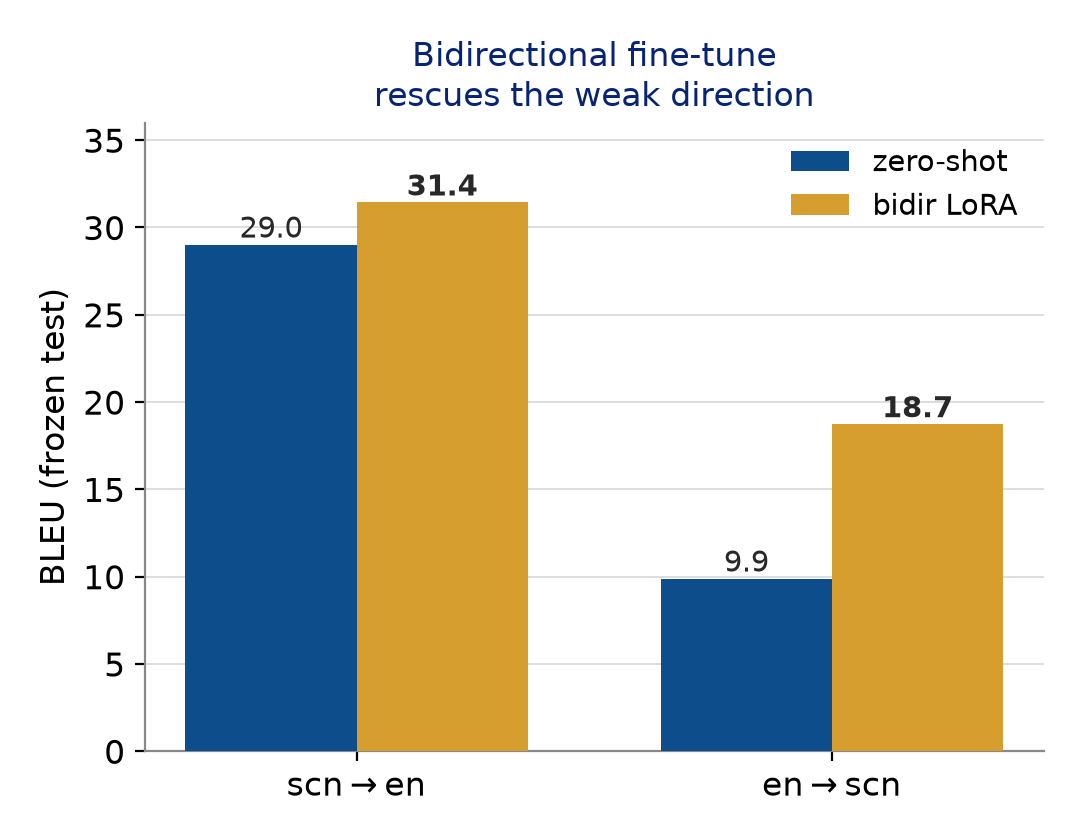
\includegraphics[width=\textwidth]{bleu_directions.png}
    \end{column}
  \end{columns}
\end{frame}

\begin{frame}{Back-translation --- turning monolingual text into data}
  \begin{columns}[t]
    \begin{column}{0.58\textwidth}
      \footnotesize
      Given a \textbf{monolingual} target corpus $\{y\}$ and a \emph{reverse} model
      $M_{t\to s}$, synthesise sources and train the forward model on real + synthetic pairs
      (Sennrich et al., 2016):
      \[
        x' = M_{t\to s}(y),\qquad
        \mathcal D^{+}=\mathcal D\,\cup\,\{(x',\,y)\}.
      \]
      The \textbf{target side $y$ is real and fluent} --- only the source is synthetic --- so the
      decoder learns better target language.\\[1mm]
      Our reverse model is the bidirectional en$\to$scn adapter; our monolingual $\{y\}$ is the
      \textbf{in-domain English} harvested from the \emph{unaligned} Arba Sicula text
      (7{,}592 sentences).
    \end{column}
    \begin{column}{0.42\textwidth}
      \begin{itemize}
        \item Exactly the lever that took the original system from BLEU 29.1 to 36.8.
        \item In-domain (literary) monolingual text $\Rightarrow$ matched to the test domain.
        \item Synthetic pairs filtered by length ratio and deduped before training.
      \end{itemize}
    \end{column}
  \end{columns}
\end{frame}

\begin{frame}{Multilingual bridging --- Italian as a pivot}
  \begin{itemize}
    \item A single multilingual model handles many directions by prepending a
          \textbf{directional token} to the source, e.g. \texttt{<2it>} (Johnson et al., 2017);
          related languages \emph{share} representations and enable zero-shot directions.
    \item Italian is far higher-resource than Sicilian and closely related. Adding
          \textbf{it--scn} data lets Italian \textbf{``bridge''} to Sicilian (Fan et al., 2020,
          \emph{beyond English-centric}) --- transferring Romance structure the English side cannot.
    \item We hold 11{,}389 it--scn pairs (+514 curated) for this auxiliary lever.
  \end{itemize}
  \vfill
  {\footnotesize\color{gray} NLLB already embodies this idea at scale; we exploit it both
  zero-shot and via fine-tuning.}
\end{frame}

% ================================================================ RESULTS
\sectiondivider{Results}{%
  \begin{itemize}
    \item Evaluation: BLEU \& chrF
    \item Our models vs the baseline
    \item Relation to the published numbers
    \item Conclusion \& outlook
  \end{itemize}}{%
  Papineni et al., \emph{BLEU}.\quad Popovi\'c, \emph{chrF}.\\
  Post, \emph{sacreBLEU} (comparable scoring).}

\begin{frame}{Evaluation --- BLEU and chrF}
  \begin{columns}[t]
    \begin{column}{0.56\textwidth}
      \footnotesize
      \textbf{BLEU}: modified $n$-gram precision with a brevity penalty,
      \[
        \mathrm{BLEU}=\underbrace{\min\!\big(1,e^{1-r/c}\big)}_{\text{brevity penalty}}\cdot
        \exp\!\Big(\textstyle\sum_{n=1}^{4} w_n\log p_n\Big).
      \]
      \textbf{chrF}: character $n$-gram F-score, robust for morphology-rich, low-resource
      languages,
      \[
        \mathrm{chrF}_\beta=(1+\beta^2)\,\frac{\mathrm{chrP}\cdot\mathrm{chrR}}{\beta^2\,\mathrm{chrP}+\mathrm{chrR}}.
      \]
    \end{column}
    \begin{column}{0.44\textwidth}
      \begin{itemize}
        \item Scored with \textbf{sacreBLEU} (\texttt{tok:13a}) for comparable numbers.
        \item Evaluated on the \textbf{frozen} 1k literary test set --- fixed once, identical
              across all runs.
        \item Sockeye rows are tokenized-space; NLLB rows are raw text (raw floor BLEU 5.27).
      \end{itemize}
    \end{column}
  \end{columns}
\end{frame}

\begin{frame}{Our models vs the baseline (scn$\to$en, our test set)}
  \begin{columns}[c]
    \begin{column}{0.62\textwidth}
      \centering
      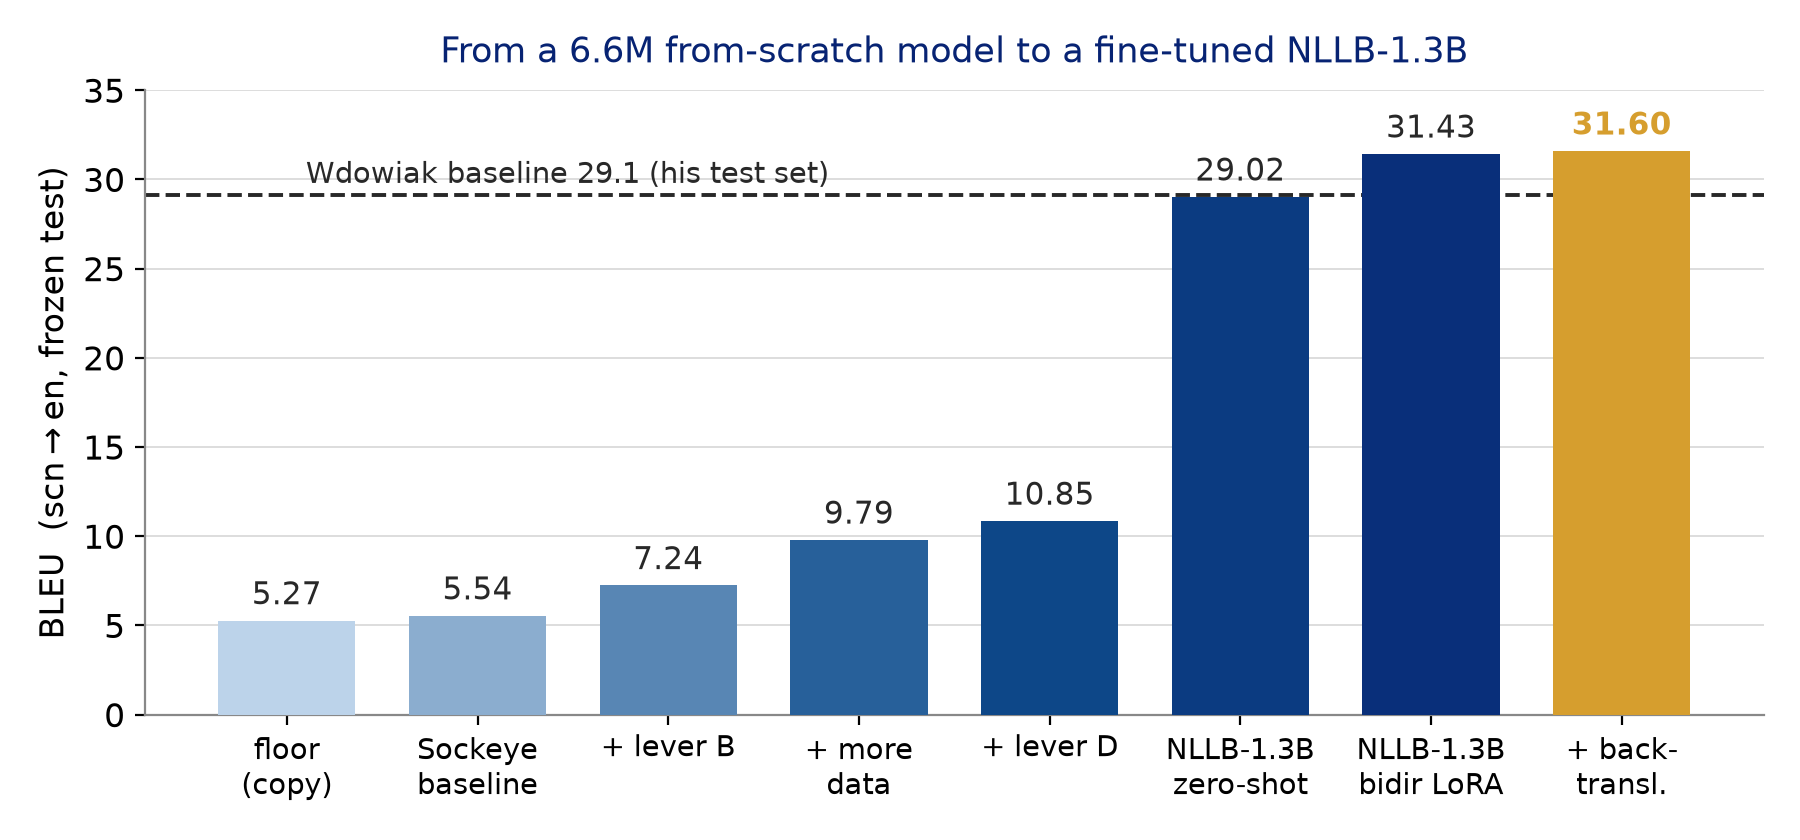
\includegraphics[width=\textwidth]{bleu_progression.png}
    \end{column}
    \begin{column}{0.38\textwidth}\footnotesize
      \begin{itemize}
        \item Each Sockeye lever \textbf{stacks}: $5.54\!\to\!10.85$ BLEU on CPU alone
              (chrF $28.3\!\to\!35.2$).
        \item The pretrained model wins decisively: \textbf{+18 BLEU} zero-shot over the best
              from-scratch model.
        \item LoRA fine-tuning adds \textbf{+2.3} on top, to \textbf{31.33} --- past the
              published baseline on our harder test.
      \end{itemize}
    \end{column}
  \end{columns}
\end{frame}

\begin{frame}{Relation to the published numbers --- not a head-to-head}
  \begin{columns}[t]
    \begin{column}{0.5\textwidth}
      Wdowiak (his in-domain test set, full recipe), BLEU:
      \begin{center}\small
      \begin{tabular}{lcc}
        \toprule & En$\to$Sc & Sc$\to$En \\\midrule
        baseline            & 25.1 & 29.1 \\
        + backtr.\ + multil.& 35.0 & 36.8 \\
        Reverse-Training    & 45.1 & 48.6 \\\bottomrule
      \end{tabular}
      \end{center}
    \end{column}
    \begin{column}{0.5\textwidth}
      \begin{itemize}
        \item \textbf{Different rulers}: his test set is in-domain and hand-selected; ours is a
              harder held-out \emph{literary} set.
        \item Still, NLLB-1.3B fine-tuned (\textbf{31.33}) already clears his published
              \emph{baseline} (29.1) \emph{on our harder test}.
        \item The next levers --- back-translation, Italian bridge --- target his
              \emph{augmented} 36.8.
      \end{itemize}
    \end{column}
  \end{columns}
  \vfill
  \centerline{\footnotesize A fair comparison runs one model on the other's test set ---
  which the NLLB experiments make possible.}
\end{frame}

\begin{frame}{Conclusion \& outlook}
  \begin{itemize}
    \item A \textbf{linear path}, fully reproduced: automated PDF$\to$parallel-text pipeline
          $\to$ small high-dropout Transformer $\to$ linguistic levers (desinences, lemma
          factors) $\to$ \textbf{NLLB-200} with LoRA and a bidirectional fine-tune.
    \item On our harder literary test set we go from BLEU \textbf{5.27} (floor) to \textbf{31.33}
          (scn$\to$en), \emph{above} the published baseline, with a usable reverse direction.
    \item \textbf{In progress}: back-translation from in-domain monolingual English; Italian
          bridging; and serving the model as a \textbf{Telegram bot}.
  \end{itemize}
  \vfill
  {\scriptsize Code, data pipeline and reproducible evaluation: \texttt{github.com/dmeoli/SicilianNMT}.}
\end{frame}

% ================================================================ Acknowledgements
\begin{frame}{Acknowledgements}
  \begin{itemize}
    \item \textbf{Arba Sicula}, \textbf{Gaetano Cipolla} and \textbf{Arthur Dieli} --- for the
          bilingual journal, the vocabulary and grammar, and for sponsoring and developing
          Sicilian language and culture; the parallel text is used by their kind permission.
    \item \textbf{Eryk Wdowiak} --- whose \emph{Tradutturi Sicilianu} and ``recipe for
          low-resource NMT'' this work builds on and reproduces.
    \item The open-source projects this stands on: \textbf{PyMuPDF}, \textbf{LaBSE}/
          sentence-transformers, \textbf{Sockeye}, \textbf{NLLB-200}, \textbf{PEFT/LoRA},
          \textbf{sacreBLEU}.
  \end{itemize}
  \vfill
  {\footnotesize\color{gray} \textit{Grazzi assai.}}
\end{frame}

% ================================================================ Thanks
{\setbeamertemplate{footline}{}
\begin{frame}[plain]
  \centering\vfill
  {\Huge\color{tan}\textbf{Grazzi}}\\[5mm]
  {\fontsize{34}{40}\selectfont\color{tan}\textbf{\textit{p'a vostra attenzioni\,!}}}\\[12mm]
  {\footnotesize\color{gray}\texttt{github.com/dmeoli/SicilianNMT}}
  \vfill
\end{frame}}

\end{document}
